% Chapter Template

\chapter{Experimental Results} % Main chapter title

\label{Chapter7} % Change X to a consecutive number; for referencing this chapter elsewhere, use \ref{ChapterX}

\lhead{Chapter 7. \emph{Experimental Results}} % Change X to a consecutive number; this is for the header on each page - perhaps a shortened title

There were a total of 16 models. The models are labelled as \texttt{(p\_)*\_{m}\_{e}}, where
\begin{enumerate}
    \item \texttt{p} $\in$ \texttt{[b, s, a]}, denotes the steps performed during preprocessing and feature extraction, where
    \begin{enumerate}
        \item \texttt{b}: \textbf{Baseline} correction was used, i.e., the mean value of a channel was subtracted from the data points (during preprocessing).
        \item \texttt{s}: The channel readings were \textbf{standardized} (during preprocessing).
        \item \texttt{a}: The features were \textbf{averaged} across all the 32 channels (during feature extraction).
    \end{enumerate}
    If neither \texttt{b} nor \texttt{s} is applied on the data, \texttt{r} (raw) is used.
    \item \texttt{m} $\in$ \texttt{[rf, xgb]}, denotes the model type used for classification, where
    \begin{enumerate}
        \item \texttt{rf}: Random Forest
        \item \texttt{xgb}: XGBoost
    \end{enumerate}
    \item \texttt{e} $\in$ \texttt{[v, a, c, p]} denotes the affect axis, where
    \begin{tasks}[label-align=left, label-offset={0mm}, label-width={5mm}, item-indent={5mm}, label-format={\bfseries}, column-sep=10mm](4)
        \task \texttt{v}: Valence
        \task \texttt{a}: Arousal
        \task \texttt{c}: Control
        \task \texttt{p}: Prediction
    \end{tasks}
    % \begin{enumerate}
    %     \item \texttt{v}: Valence
    %     \item \texttt{a}: Arousal
    %     \item \texttt{c}: Control
    %     \item \texttt{p}: Prediction
    % \end{enumerate}
\end{enumerate}

\begin{table}[t]
\caption{Accuracy in Percentage} % title of Table
\centering
\hspace*{-1.8cm}
\begin{tabular}{cc|c|c|c|c|c|c|c|c|}
\cline{3-10}
                                                &     & \multicolumn{4}{c|}{Train}               & \multicolumn{4}{c|}{Test}                \\ \cline{3-10} 
                                                &     & Valence & Arousal & Control & Prediction & Valence & Arousal & Control & Prediction \\ \hline
\multicolumn{1}{|c|}{}                          & rf  & 88.44   & 88.88   & 88.05   & 85.16      & 82.76   & 85.50   & 86.08   & 80.87      \\ \cline{2-10} 
\multicolumn{1}{|c|}{\multirow{-2}{*}{r}} &
  xgb &
  89.97 &
  86.61 &
  90.33 &
  86.42 &
  \cellcolor[HTML]{FFFC9E}\textbf{85.80} &
  85.70 &
  \cellcolor[HTML]{FFFC9E}\textbf{87.73} &
  83.51 \\ \hline
\multicolumn{1}{|c|}{}                          & rf  & 79.01   & 79.10   & 79.10   & 73.20      & 67.87   & 68.15   & 70.17   & 62.87      \\ \cline{2-10} 
\multicolumn{1}{|c|}{\multirow{-2}{*}{b}}       & xgb & 82.47   & 80.85   & 80.58   & 77.21      & 71.27   & 70.21   & 72.54   & 66.95      \\ \hline
\multicolumn{1}{|c|}{}                          & rf  & 88.71   & 89.60   & 89.04   & 85.54      & 81.59   & 83.85   & 86.01   & 78.57      \\ \cline{2-10} 
\multicolumn{1}{|c|}{\multirow{-2}{*}{s}} &
  xgb &
  \cellcolor[HTML]{FFFC9E}\textbf{90.92} &
  \cellcolor[HTML]{FFFC9E}\textbf{92.33} &
  \cellcolor[HTML]{FFFC9E}\textbf{91.67} &
  \cellcolor[HTML]{FFFC9E}\textbf{90.55} &
  84.68 &
  \cellcolor[HTML]{FFFC9E}\textbf{87.56} &
  86.84 &
  \cellcolor[HTML]{FFFC9E}\textbf{85.60} \\ \hline
\multicolumn{1}{|c|}{}                          & rf  & 88.02   & 90.27   & 89.13   & 85.87      & 80.29   & 84.50   & 85.64   & 79.23      \\ \cline{2-10} 
\multicolumn{1}{|c|}{\multirow{-2}{*}{b\_s}} &
  xgb &
  \cellcolor[HTML]{FFFC9E}\textbf{90.92} &
  \cellcolor[HTML]{FFFC9E}\textbf{92.33} &
  \cellcolor[HTML]{FFFC9E}\textbf{91.67} &
  \cellcolor[HTML]{FFFC9E}\textbf{90.55} &
  84.68 &
  \cellcolor[HTML]{FFFC9E}\textbf{87.56} &
  86.84 &
  \cellcolor[HTML]{FFFC9E}\textbf{85.60} \\ \hline
\multicolumn{1}{|c|}{}                          & rf  & 72.66   & 76.59   & 76.65   & 67.72      & 64.35   & 70.62   & 72.75   & 62.63      \\ \cline{2-10} 
\multicolumn{1}{|c|}{\multirow{-2}{*}{a\_r}}    & xgb & 73.95   & 76.81   & 79.85   & 74.13      & 69.32   & 72.61   & 76.86   & 70.93      \\ \hline
\multicolumn{1}{|c|}{}                          & rf  & 67.31   & 68.02   & 67.33   & 63.16      & 56.56   & 59.72   & 60.00   & 53.38      \\ \cline{2-10} 
\multicolumn{1}{|c|}{\multirow{-2}{*}{a\_b}}    & xgb & 64.36   & 65.87   & 66.45   & 62.40      & 55.54   & 58.18   & 59.44   & 54.20      \\ \hline
\multicolumn{1}{|c|}{}                          & rf  & 66.28   & 67.70   & 67.87   & 66.05      & 58.00   & 61.19   & 60.75   & 57.35      \\ \cline{2-10} 
\multicolumn{1}{|c|}{\multirow{-2}{*}{a\_s}}    & xgb & 65.20   & 66.93   & 67.96   & 64.44      & 58.48   & 61.23   & 61.40   & 56.91      \\ \hline
\multicolumn{1}{|c|}{}                          & rf  & 66.27   & 68.43   & 67.67   & 66.60      & 57.32   & 62.11   & 60.37   & 57.56      \\ \cline{2-10} 
\multicolumn{1}{|c|}{\multirow{-2}{*}{a\_b\_s}} & xgb & 65.20   & 66.94   & 67.96   & 64.44      & 58.48   & 61.23   & 61.40   & 56.91      \\ \hline
\end{tabular}
\end{table}


\begin{table}[t]
\caption{Precision and Recall of Test Dataset} % title of Table
\centering
\hspace*{-1.8cm}
\begin{tabular}{cc|c|c|c|c|c|c|c|c|}
\cline{3-10}
 &
   &
  \multicolumn{4}{c|}{Precision} &
  \multicolumn{4}{c|}{Recall} \\ \cline{3-10} 
 &
   &
  Valence &
  Arousal &
  Control &
  Prediction &
  Valence &
  Arousal &
  Control &
  Prediction \\ \hline
\multicolumn{1}{|c|}{} &
  rf &
  0.83 &
  0.86 &
  0.87 &
  0.83 &
  0.83 &
  0.85 &
  0.86 &
  0.81 \\ \cline{2-10} 
\multicolumn{1}{|c|}{\multirow{-2}{*}{r}} &
  xgb &
  \cellcolor[HTML]{FFFC9E}\textbf{0.86} &
  0.86 &
  \cellcolor[HTML]{FFFC9E}\textbf{0.88} &
  0.85 &
  \cellcolor[HTML]{FFFC9E}\textbf{0.86} &
  0.86 &
  \cellcolor[HTML]{FFFC9E}\textbf{0.88} &
  0.84 \\ \hline
\multicolumn{1}{|c|}{} &
  rf &
  0.69 &
  0.69 &
  0.70 &
  0.67 &
  0.68 &
  0.68 &
  0.70 &
  0.63 \\ \cline{2-10} 
\multicolumn{1}{|c|}{\multirow{-2}{*}{b}} &
  xgb &
  0.72 &
  0.71 &
  0.73 &
  0.69 &
  0.71 &
  0.70 &
  0.73 &
  0.67 \\ \hline
\multicolumn{1}{|c|}{} &
  rf &
  0.83 &
  0.84 &
  0.86 &
  0.84 &
  0.82 &
  0.84 &
  0.86 &
  0.79 \\ \cline{2-10} 
\multicolumn{1}{|c|}{\multirow{-2}{*}{s}} &
  xgb &
  0.85 &
  \cellcolor[HTML]{FFFC9E}\textbf{0.88} &
  0.87 &
  \cellcolor[HTML]{FFFC9E}\textbf{0.86} &
  0.85 &
  \cellcolor[HTML]{FFFC9E}\textbf{0.88} &
  0.87 &
  \cellcolor[HTML]{FFFC9E}\textbf{0.86} \\ \hline
\multicolumn{1}{|c|}{} &
  rf &
  0.82 &
  0.85 &
  0.86 &
  0.84 &
  0.80 &
  0.85 &
  0.86 &
  0.79 \\ \cline{2-10} 
\multicolumn{1}{|c|}{\multirow{-2}{*}{b\_s}} &
  xgb &
  0.85 &
  \cellcolor[HTML]{FFFC9E}\textbf{0.88} &
  0.87 &
  \cellcolor[HTML]{FFFC9E}\textbf{0.86} &
  0.85 &
  \cellcolor[HTML]{FFFC9E}\textbf{0.88} &
  0.87 &
  \cellcolor[HTML]{FFFC9E}\textbf{0.86} \\ \hline
\multicolumn{1}{|c|}{} &
  rf &
  0.67 &
  0.71 &
  0.73 &
  0.70 &
  0.64 &
  0.71 &
  0.73 &
  0.63 \\ \cline{2-10} 
\multicolumn{1}{|c|}{\multirow{-2}{*}{a}} &
  xgb &
  0.70 &
  0.74 &
  0.77 &
  0.74 &
  0.69 &
  0.73 &
  0.77 &
  0.71 \\ \hline
\multicolumn{1}{|c|}{} &
  rf &
  0.58 &
  0.60 &
  0.60 &
  0.57 &
  0.57 &
  0.60 &
  0.60 &
  0.53 \\ \cline{2-10} 
\multicolumn{1}{|c|}{\multirow{-2}{*}{a\_b}} &
  xgb &
  0.56 &
  0.58 &
  0.59 &
  0.56 &
  0.56 &
  0.58 &
  0.59 &
  0.54 \\ \hline
\multicolumn{1}{|c|}{} &
  rf &
  0.59 &
  0.61 &
  0.61 &
  0.61 &
  0.58 &
  0.61 &
  0.61 &
  0.57 \\ \cline{2-10} 
\multicolumn{1}{|c|}{\multirow{-2}{*}{a\_s}} &
  xgb &
  0.59 &
  0.61 &
  0.62 &
  0.58 &
  0.58 &
  0.61 &
  0.61 &
  0.57 \\ \hline
\multicolumn{1}{|c|}{} &
  rf &
  0.58 &
  0.62 &
  0.61 &
  0.61 &
  0.57 &
  0.62 &
  0.60 &
  0.58 \\ \cline{2-10} 
\multicolumn{1}{|c|}{\multirow{-2}{*}{a\_b\_s}} &
  xgb &
  0.59 &
  0.61 &
  0.62 &
  0.58 &
  0.58 &
  0.61 &
  0.61 &
  0.57 \\ \hline
\end{tabular}
\end{table}

\section {Tables}

The tables above show the train and test accuracy, and precision and recall on test set, for each of the variation in the pipeline. We see that XGBoost performs a bit better than Random Forest in all the cases. Also, features extracted from raw data gives nearly as good a result as standardised and baseline-removed data. On the test dataset, both \texttt{r} and \texttt{b\_s} are equally strong, while \texttt{b\_s} works better on the train dataset. 

\section {Plots}
\subsection{\texttt{b\_s\_\_xgb}}
\begin{figure}[H]
\centering
\hspace*{-1.5cm}
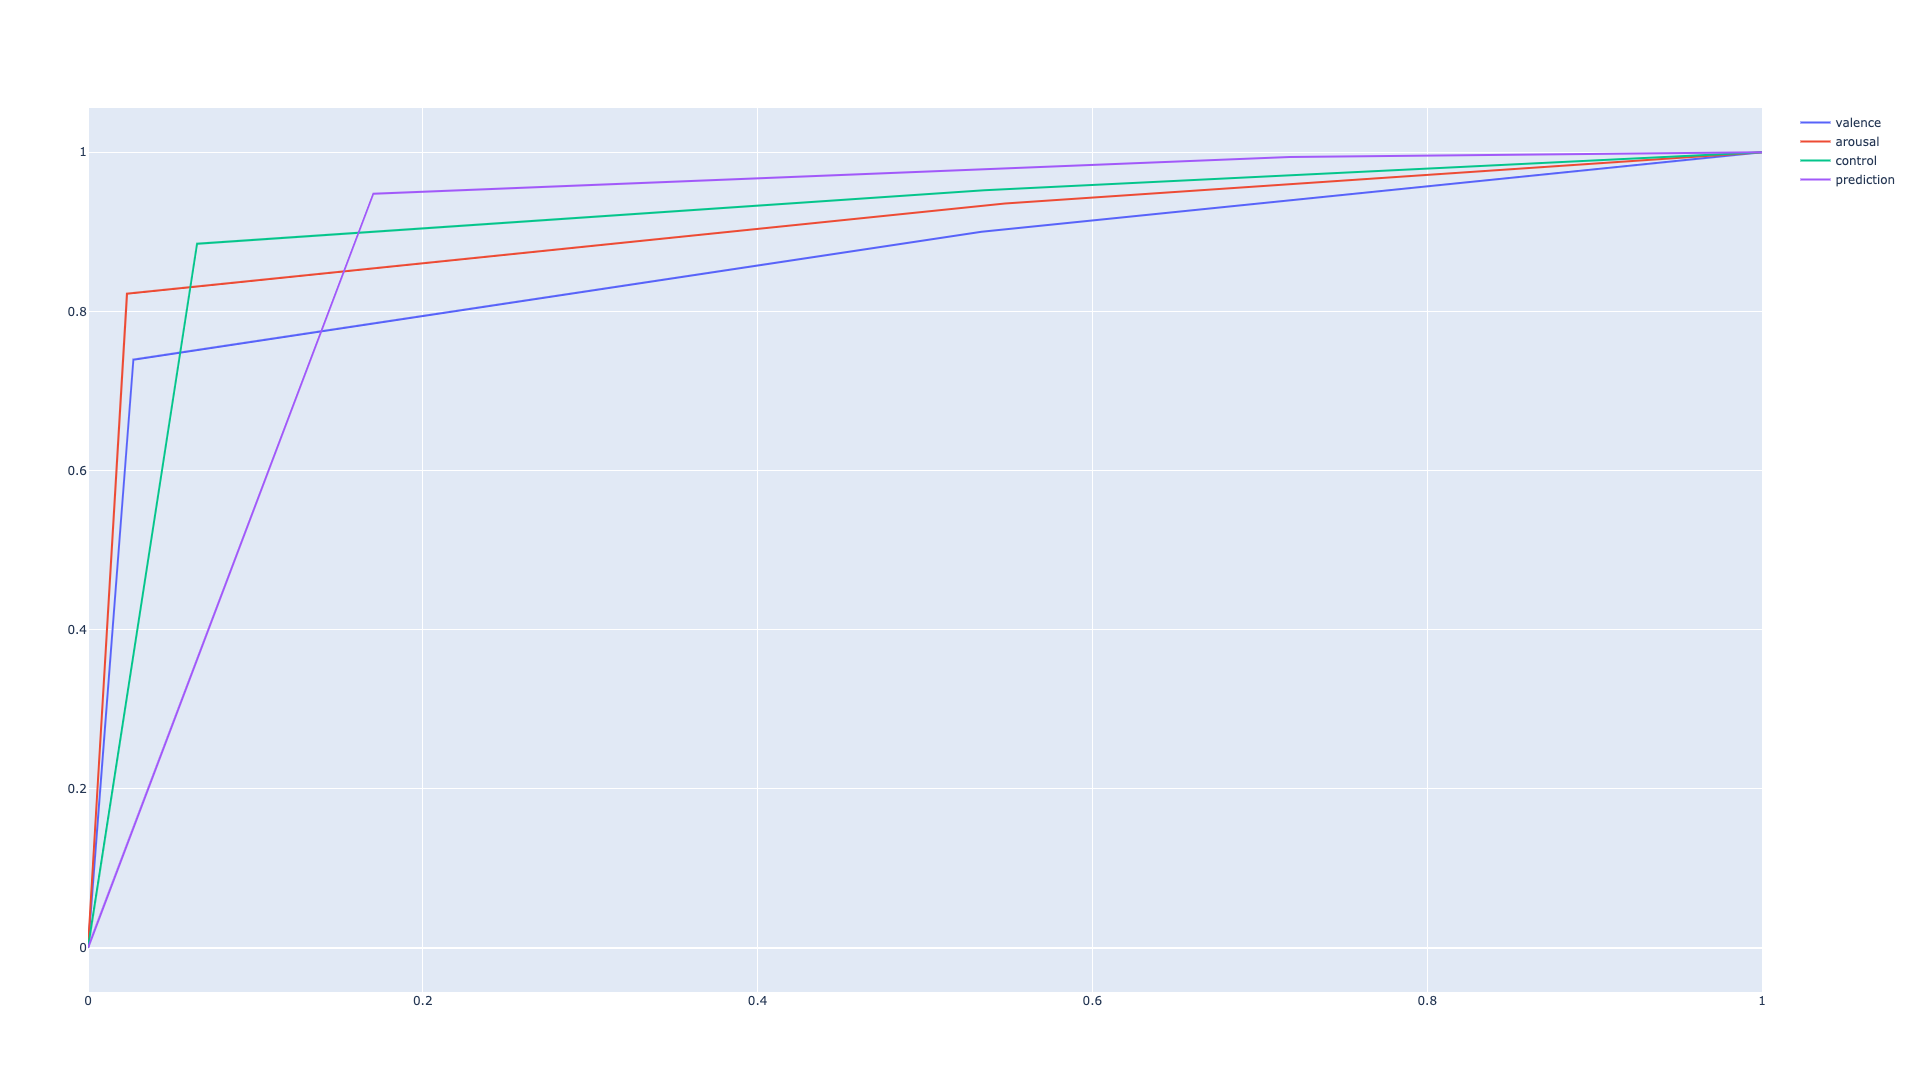
\includegraphics[height=10cm]{res_roc__b_s_xgb.png}
\caption{ROC Curve}
\label{fig-7-1}
\end{figure}

\begin{figure}[H]
\centering
\hspace*{-1.5cm}
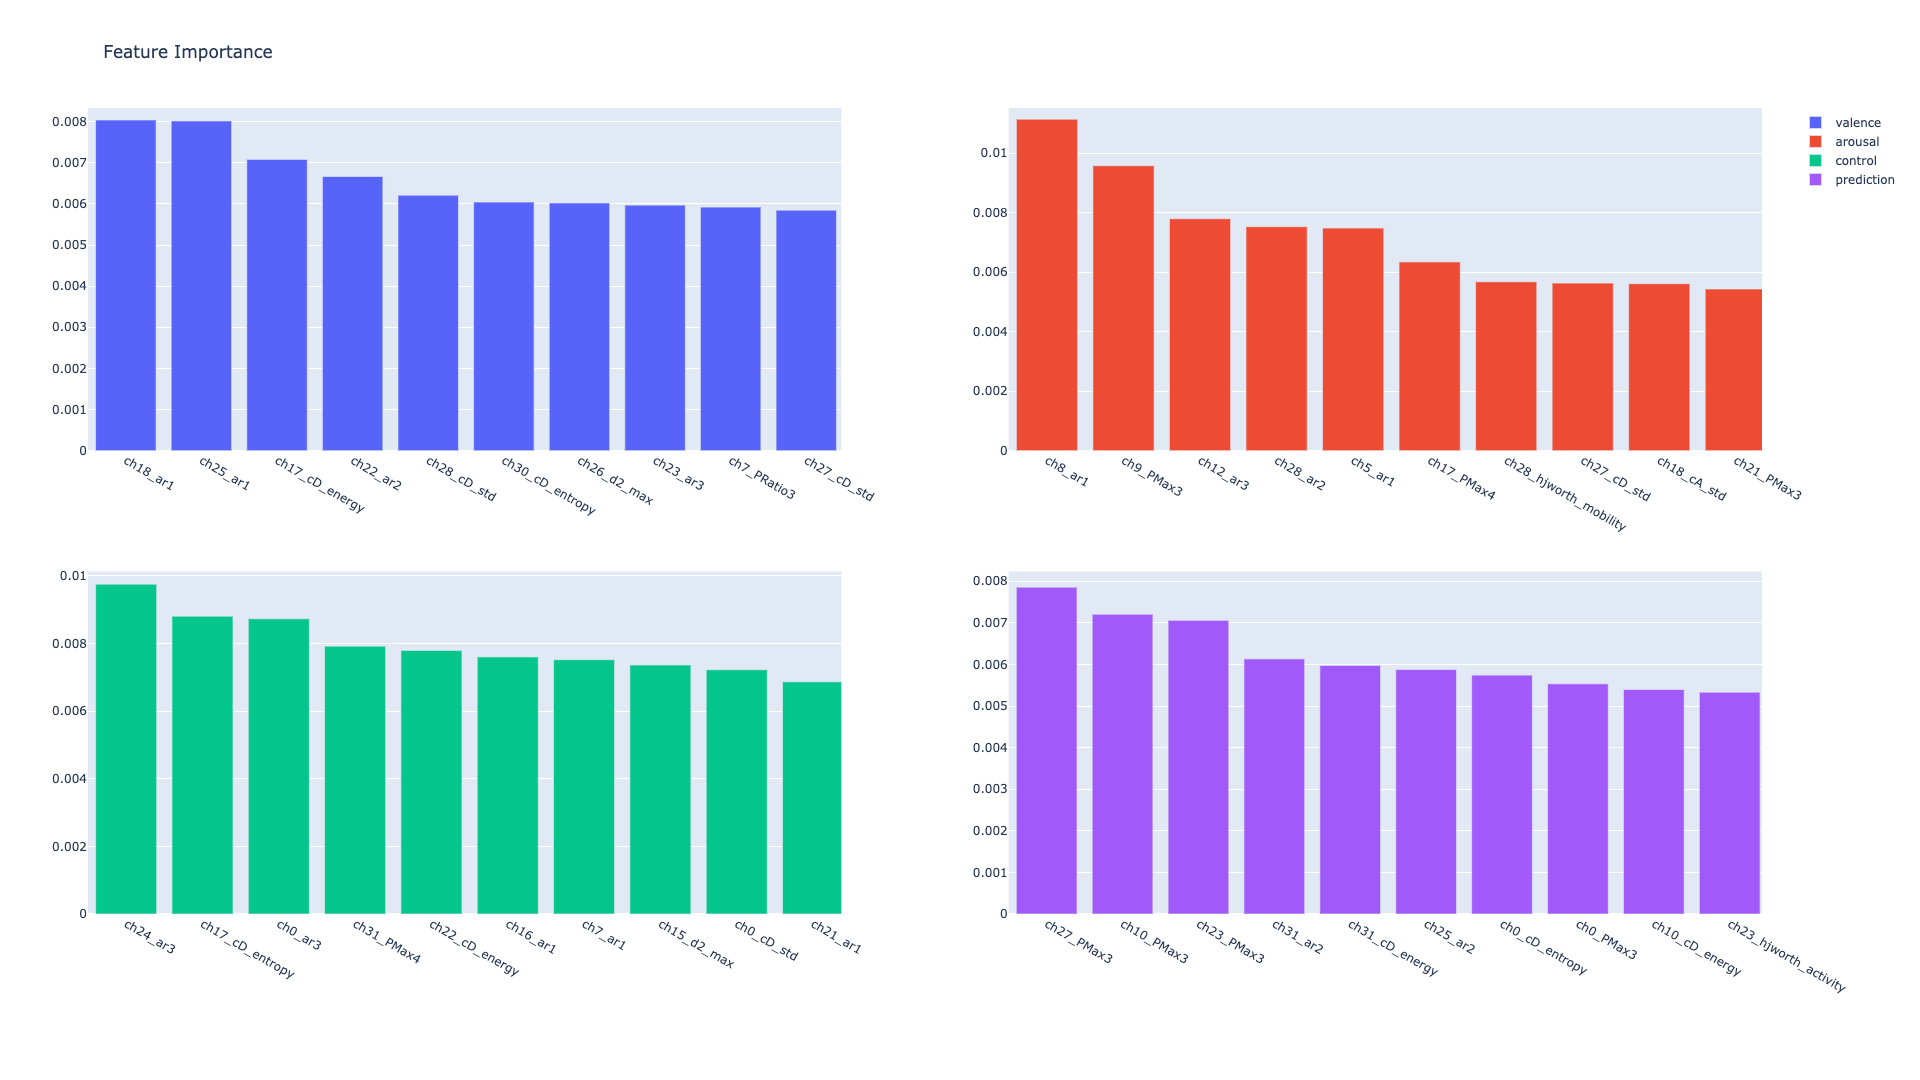
\includegraphics[height=10cm]{res_feature_importance__b_s_xgb.png}
\caption{Feature Importances}
\label{fig-7-2}
\end{figure}

\subsection{\texttt{r\_\_xgb}}
\begin{figure}[H]
\centering
\hspace*{-1.5cm}
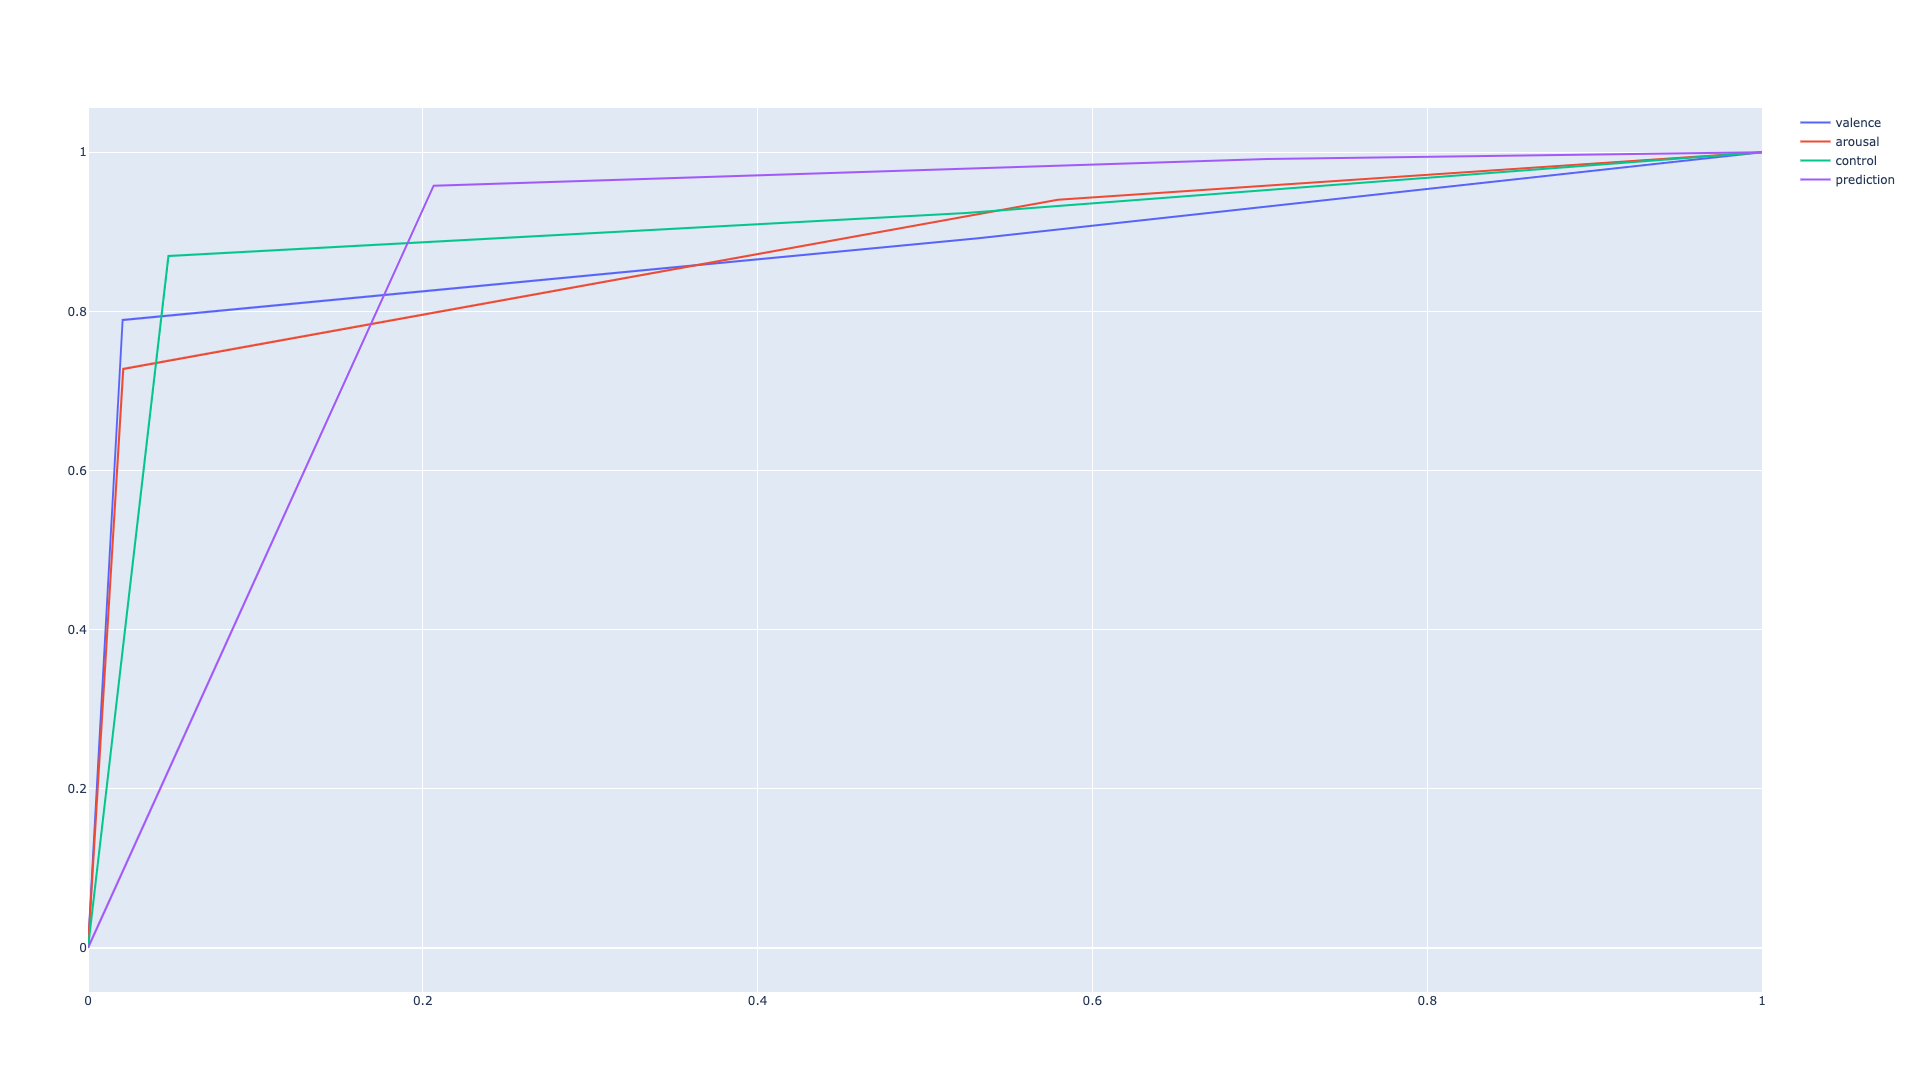
\includegraphics[height=10cm]{res_roc__r_xgb.png}
\caption{ROC Curve}
\label{fig-7-3}
\end{figure}

\begin{figure}[H]
\centering
\hspace*{-1.5cm}
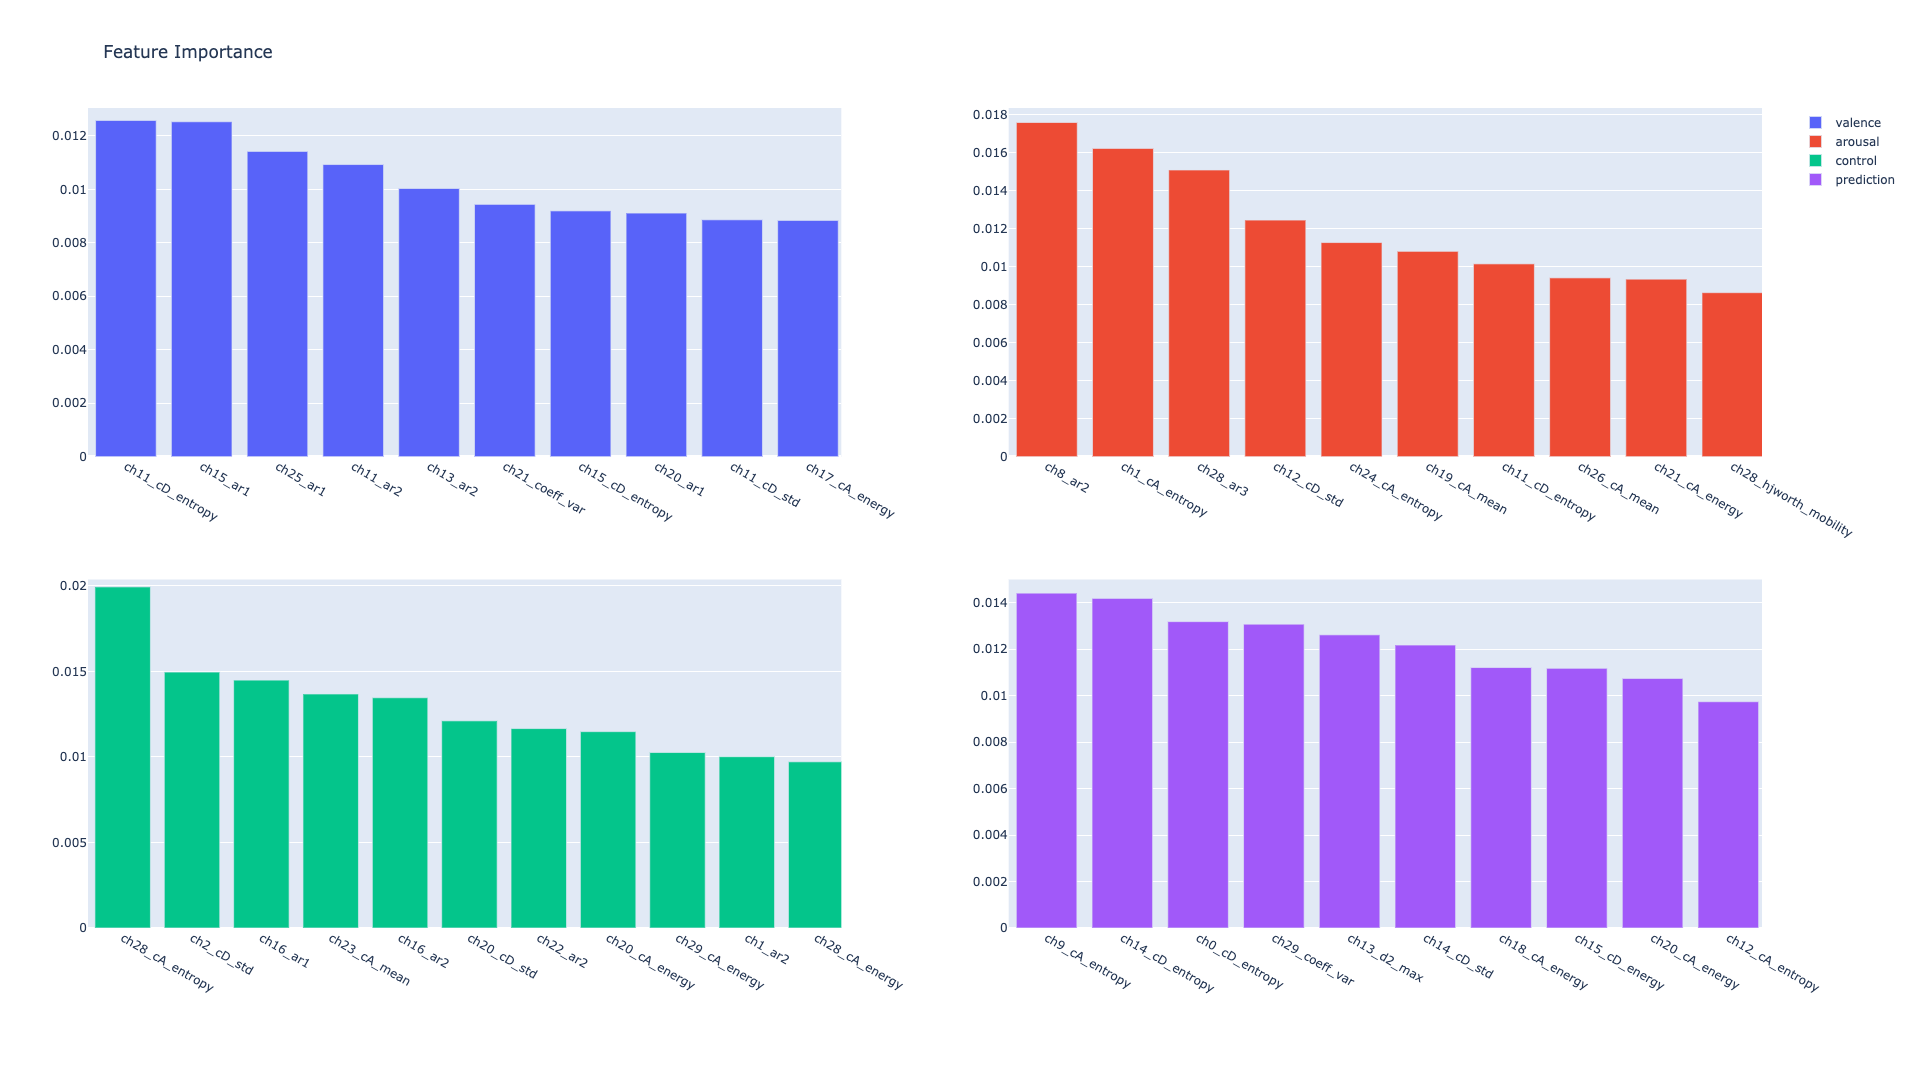
\includegraphics[height=10cm]{res_feature_importance__r_xgb.png}
\caption{Feature Importances}
\label{fig-7-4}
\end{figure}
